% 原文 pp.188–194（印刷 pp.1306–1312）
% 承接第 13 讲第 2 部分：本文件自 §13.6 起，故不写 \section

% ===== 原文 p.188 =====

例如，我们可以这样构造一对 $h^{1,1}=2$ 的 Calabi--Yau 流形：从规范群 $G=U(1)\times U(1)$ 以及形如 $W=PF(A_i)$ 的超势出发。
只要设置得当，其中一个 $U(1)$ 就把我们带入射影簇（projective variety）$X$ 与 $X'$ 的世界；而通过改变另一个 $U(1)$ 的矩映射（moment map），我们便可以在 $X$ 与 $X'$ 之间做出一个「flop」，它与上面关于四个手征超场 $A_i$、$B_j$ 的讨论十分相似。

% [Tutor Note: 「flop」与 Fayet--Iliopoulos 参数的关系值得说清。线性 $\sigma$ 模型中 $U(1)$ 的 FI 参数 $r$ 与 $\theta$ 角组合成复参数 $t$；把 (13.8) 的临界点方程与 p.190 的分量形式 $0=-ir+\frac{\theta}{2\pi}-\frac{in}{2\pi}\ln(\sigma/\mu)$ 对照，即可定出本文的约定 $t=\frac{\theta}{2\pi}-ir$（实部是 $\theta$ 角、虚部是 FI 参数，二者地位并不对称）。$r$ 穿过 $0$ 时，$D$ 项条件所定义的商空间从一个相「翻转」到另一个相，这正是 flop 的线性 $\sigma$ 模型实现。这一约定还有一个可检验的推论：p.191 末尾的奇点判据 $t-\frac{i}{2\pi}\sum_i q_i\ln|q_i|=0$ 是纯虚的，故奇点只落在 $\theta\equiv0\pmod{2\pi}$、$r=-\frac{1}{2\pi}\sum_i q_i\ln|q_i|$ 处，而不会在 $\theta$ 方向移动；若把 $t$ 的实虚部记反，就会得出「奇点随 $\theta$ 平移」的错误结论。另：原文此句作 ``the four chiral superfields fields $A_i$ and $B_j$''，``fields'' 重出，应属笔误，译文按「四个手征超场」处理。]

\subsection{$c_1\ne0$ 的情形}
% 原文 §13.6：Cases in which $c_1\ne0$

现在我们要考虑 $R$ 对称性反常的线性 $\sigma$ 模型（linear sigma model），因此预期存在非平凡的重整化群流。

\subsubsection{负 $\beta$ 函数}
% 原文 §13.6.1：Negative $\beta$-function

我们从负 $\beta$ 函数的情形开始；对非线性 $\sigma$ 模型而言，这对应于满足 $c_1(TX)>0$ 的目标空间 $X$。
这类例子可以完全照旧构造：让 $U(1)$ 作用在 $n+1$ 个场 $A_i,P$ 上，但这一次赋给 $P$ 荷 $-k$，并取超势 $W=P\cdot F$，其中 $F$ 是 $k$ 次齐次多项式。
该 $\sigma$ 模型的 $\beta$ 函数在 $k<n$、$k=n$、$k>n$ 时依次为负、零、正。

% [Tutor Note: 「负 $\beta$ 函数 $\Leftrightarrow c_1(TX)>0$」用的是 $\beta=\mu\,dg/d\mu$ 的约定，即负 $\beta$ 函数就是渐近自由；其几何判据是目标空间的 Ricci 形式正定，等价于 $c_1(TX)>0$（Fano）。若换成 $\beta=-\mu\,dg/d\mu$ 的相反约定（部分文献如此），则整段关于 $k\lessgtr n$ 的结论要全部反号，这是读文献时最易翻车之处。另请注意本段有两处结论都以 $k\ne n$ 为前提，而 $k=n$（Calabi--Yau）恰是 $c_1=0$、$\beta=0$ 的临界情形，此时既无红外不动点也无紫外不动点，故被排除在讨论之外。]

对 $k\ne n$，尽管经典地看 $r=0$ 处仍有奇点，量子理论在 $t$ 柱面（$t$-cylinder）上却没有奇点。
（这一点通过分析大 $\sigma$ 处的行为来证明，我们马上就会做。）
对 $k\ne n$，柱面上存在非平凡的重整化群流。
该流是全纯的、无奇点的，因此它是柱面上「向下」或「向上」的匀速流，方向取决于 $n-k$ 的符号。

\begin{figure}[htbp]
  \centering
  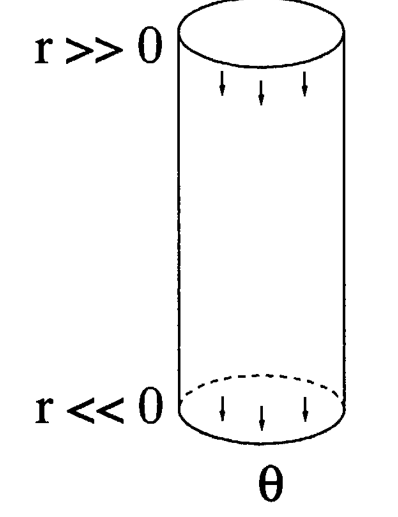
\includegraphics[width=0.30\textwidth]{figs/fig_p188_1.png}
  \caption{$t$ 柱面：竖直方向为 $r$，绕柱的圆周方向为 $\theta$ 角。顶端标注 $r\gg0$（$\sigma$ 模型端），底端标注 $r\ll0$（Landau--Ginzburg 端），柱面上的箭头示意重整化群流的方向。（原文 Figure 6，p.188）}
  \label{fig:p188-1}
\end{figure}

当我们重复先前的分析时，会发现来自四维 $R$ 对称性的那个 $R$ 对称性是反常的，而来自缺失方向转动的那个 $R$ 对称性则无反常。

经典分析同样可以重复：对 $r\gg0$，我们得到由 $\mathbf{P}^{n-1}$ 中的 $\{F=0\}$ 描述的经典真空空间，并预期该超曲面上的非线性 $\sigma$ 模型是我们理论的良好近似。
当 $k<n$ 时，这个超曲面具有正的第一 Chern 类，因此从非线性 $\sigma$ 模型出发，我们预期得到一个定义良好的量子场论。
另一方面，由于 $k<n$，该 $\sigma$ 模型在红外是不稳定的。
红外流会把我们带离 $\sigma$ 模型，趋向我们在 $r\to-\infty$ 极限处将找到的理论。
注意该 $\sigma$ 模型的目标空间是 $(n-2)$ 维的，因此在 $k<n$ 时，紫外极限下的有效中心荷为 $\widehat{c}=n-2$。

另一方面，若 $r\ll0$，则经典真空空间上 $P\ne0$ 而 $A_i=\sigma=0$。
给 $P$ 一个非零期望值把 $U(1)$ 破缺为 $\mathbf{Z}_k$，并且（在

% ===== 原文 p.189 =====

$r\to-\infty$ 极限下）我们得到一个 Landau--Ginzburg 轨形（orbifold），其有效相互作用为
\[
W_{\rm eff}(A_i)=F(A_i).
\]
该模型的中心荷为
\[
\widehat{c}=n\Bigl(1-\frac{2}{k}\Bigr).
\]
当 $k<n$ 时它小于 $n-2$。
我们稍后将论证：对 $k<n$，Landau--Ginzburg 理论正是从 $\sigma$ 模型出发的重整化群流的红外极限；而它的中心荷比 $\sigma$ 模型的小这一事实，恰好说明了 Zamolodchikov 的一个一般定理——该定理断言中心荷沿重整化群流总是减小：
\[
c_{\rm IR}\le c_{\rm UV}.
\]

% [Tutor Note: 作者在 $c$ 与 $\widehat{c}$ 之间来回切换，必须按 $c=3\widehat{c}$ 换算（二维 $\mathcal N=2$ 超共形代数的标准归一化：$W=\Phi^k$ 的 Landau--Ginzburg 模型有 $\widehat{c}=1-2/k$，对应 $A_{k-1}$ 极小模型的 $c=3(k-2)/k$）。因此 $c_{\rm IR}\le c_{\rm UV}$ 与 $\widehat{c}_{\rm IR}\le\widehat{c}_{\rm UV}$ 等价，本页的数值比较（如 $\widehat{c}=n(1-2/k)<n-2$）不受影响；但切勿把某页的 $\widehat{c}$ 与另一页的 $c$ 直接相减，否则会差一个因子 3。另需注意：$\widehat{c}=n(1-2/k)$ 是 $n$ 个手征超场、超势次数为 $k$ 的 LG 轨形的值，其中的 $P$ 场因获得质量而不计入；轨形化（orbifold）本身不改变中心荷。]

该定理背后的直观是：中心荷衡量理论中自由度的总数。
随着向红外流动，有质量的自由度被「积掉」（integrated out），不再对中心荷有贡献，因此中心荷只可能减小。

我们将看到，对 $k<n$，Landau--Ginzburg 模型只是红外流可能达到的结果之一。
事实上在 $r=-\infty$ 处还有 $n-k$ 个另外的真空态，它们有质量间隙（mass gap），经典上看不见，需要用单圈计算才能得到。
由于有质量，它们的 $\widehat{c}=0$，当然小于 $n-2$。

\subsubsection{$\mathbf{CP}^{n-1}$ 模型}
% 原文 §13.6.2：The $\mathbf{CP}^{n-1}$ model

我们所考虑的情形的一个极端例子是 $k=0$，即没有 $P$ 场、也没有超势的情形。
这是一个带 $n$ 个自由带电超场 $A_1,\dots,A_n$（荷全为 $1$）的 $U(1)$ 规范理论。
$D$ 项取如下形式
\[
D=\sum_i|A_i|^2-r.
\]
令它为零再除以 $U(1)$，我们便得到（对 $r\gg0$）先前某一讲中研究过的超对称 $\mathbf{CP}^{n-1}$ 模型。
在回到一般情形之前，详细重审这个例子将极有启发。

乍看之下，这个 $\mathbf{CP}^{n-1}$ 模型在 $r\to-\infty$ 极限下似乎根本没有超对称真空，因为矩映射是严格正的。
然而，在这个极限下根本不存在超对称真空是不可能的。
超对称指标 $\operatorname{Tr}(-1)^F$ 提供了阻碍。（我在去年秋季的讲座中讨论过这个指标及其推广——椭圆亏格。）
对大的正 $r$ 计算，这个指标与 $\mathbf{CP}^{n-1}$ 的 Euler 特征数相等，即为 $n$。
超对称指标在 $r$ 的形变下必须不变，因此即使 $r$ 很大且为负，也必须存在 $n$ 个超对称真空。
我们总得在某处找到它们！

要看清究竟发生了什么，我们必须更仔细地考察量子力学。
对 $r\to-\infty$ 极限的经典处理在场空间的任何紧区域中都成立，因此，如果对任意负的 $r$ 存在经典上看不见的量子力学真空，那么当 $r\to-\infty$ 时它们必须以「跑到场空间无穷远」的方式从经典视野中消失。
所以我们必须再次考察大 $\sigma$ 处的量子力学行为。
对我们的 $\mathbf{CP}^{n-1}$ 模型，玻色子势取如下形式
\[
V=\frac{e^2}{2}D^2+|\sigma|^2\sum_i|A_i|^2.
\]

% ===== 原文 p.190 =====

该理论在 $r\ll0$ 时是弱耦合的。

若 $|\sigma|\to\infty$ 会怎样？
与先前一样，此时场 $A_i$ 将获得质量，可以被积掉，从而得到一个阿贝尔规范理论作为有效理论，其拉氏量为
\[
\mathcal{L}_{\rm eff}=\int d^2x\,d^4\theta\,\frac{1}{2e^2}\overline{\Sigma}\Sigma
+\Bigl(\int d^2x\,d\bar\theta^+\,d\theta^-\,\widetilde{\mathcal{W}}_{\rm eff}(\Sigma)+{\rm c.c.}\Bigr).
\]
有效扭曲超势（twisted superpotential）依赖于重整化质量标度 $\mu$，而我们断言它取如下新颖的（破坏 $R$ 对称性的）形式
\begin{equation}
  \tag{13.8}
  \label{eq:13-8}
  \widetilde{\mathcal{W}}_{\rm eff}(\Sigma)=t\Sigma+\frac{in}{2\pi}\bigl(\Sigma-\Sigma\ln(\Sigma/\mu)\bigr),
\end{equation}
我们将通过下面的单圈计算来验证它。
注意，在 (13.8) 中改变对数的选取，可以由把 $t$ 的值改变一个整数来补偿；这样的改变对物理没有影响。
当然，为了使 $\widetilde{\mathcal{W}}_{\rm eff}$ 中的对数有定义，我们必须让 $\Sigma$ 远离零，这与我们假设 $\sigma$ 很大是一致的。

% [Tutor Note: 「把 $t$ 改变一个整数」可以显式验证：绕一圈 $\ln\Sigma\to\ln\Sigma+2\pi i$ 使 $\widetilde{\mathcal{W}}_{\rm eff}\to\widetilde{\mathcal{W}}_{\rm eff}+\frac{in}{2\pi}(-\Sigma\cdot2\pi i)=\widetilde{\mathcal{W}}_{\rm eff}+n\Sigma$，即 $t\to t+n$，而 $n$ 是带电场的个数、必为整数，等价于 $\theta\to\theta+2\pi n$。这里应当警惕两点：(i) 移动的是 $t$ 的实部（$\theta$），不是虚部（$r$），因为 $\frac{in}{2\pi}\Sigma\cdot2\pi i$ 的符号由 $+i$ 与 $+2\pi i$ 相乘决定，极易写反；(ii) 若超势中写成 $\Sigma\ln\Sigma$ 而非 $\Sigma\ln(\Sigma/\mu)$，则 $t$ 的平移还会带上 $\ln\mu$，重整化标度的意义就丢失了——这正是作者保留 $\mu$ 的原因。]

有了扭曲超势中的这一新项，$\widetilde{\mathcal{W}}_{\rm eff}$ 的临界点方程为
\[
0=t-\frac{in}{2\pi}\ln(\Sigma/\mu),
\]
或者写成分量形式，
\[
0=-ir+\frac{\theta}{2\pi}-\frac{in}{2\pi}\ln(\sigma/\mu)\pmod 1.
\]
它有 $n$ 个解
\begin{equation}
  \tag{13.9}
  \label{eq:13-9}
  \sigma=\mu\exp\Bigl(-\frac{2\pi r}{n}-\frac{i\theta}{n}+\frac{2\pi ik}{n}\Bigr),\qquad
  k=0,\dots,n-1,
\end{equation}
对应于 $r\to-\infty$ 极限下 $n$ 个不同的真空。
$n$ 当然正是预期的数目，即 $\mathbf{CP}^{n-1}$ 的 Euler 特征数。
注意当 $r\to-\infty$ 时 $|\sigma|$ 确实很大，因此推导这些真空时所作的假设成立。
这 $n$ 个真空在 $r\to-\infty$ 时跑向场空间的无穷远，而它们的存在又依赖于单圈量子修正，这两点合起来解释了为什么经典上看不见它们。

对数的另一个非常重要的推论是：当 $\sigma\to\infty$ 时，量子理论中的能量按 $|\ln\sigma|^2$ 增长。
因此特别地，低能态被限制在场空间的一个有界区域内，从而对柱面上 $t$ 的任何取值，真空行为都不会出现奇点。
我们将会看到，$n\ne k$ 的模型都有这样的对数，因此它们在整个 $t$ 柱面上都是非奇异的。

\subsubsection{单圈计算}
% 原文 §13.6.3：The 1-loop calculation

要理解有效扭曲超势中 $\frac{in}{2\pi}\bigl(\Sigma-\Sigma\ln(\Sigma/\mu)\bigr)$ 这一项的起源，注意它的存在等价于有效拉氏量含有一项
\[
\int d^2x\,r_{\rm eff}D,
\]
其中
\[
r_{\rm eff}=r+\frac{n}{2\pi}\ln(|\sigma|/\mu).
\]

% ===== 原文 p.191 =====

在这个理论中，$D=\sum_i\overline{A}_iA_i-r$。
经典地，对大 $\sigma$ 有 $A_i=0=\overline{A}_iA_i$，但量子地，$\overline{A}_iA_i$ 在大 $\sigma$ 处有期望值；这个期望值在有效的经典描述中可以解释为 $-r$ 的一个平移。
因此我们需要借助单圈图来计算 $\overline{A}A$ 的期望值

\begin{figure}[htbp]
  \centering
  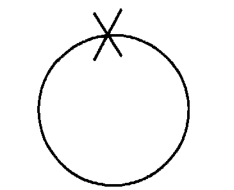
\includegraphics[width=0.16\textwidth]{figs/fig_p191_1.png}
  \caption{计算 $\langle\overline{A}_iA_i\rangle$ 的单圈图：一个闭合的玻色子圈，顶部的叉号代表 $\overline{A}A$ 算符插入（外线）。该图的贡献即下式的动量积分。（原文 Figure 7，p.191）}
  \label{fig:p191-1}
\end{figure}

它对 $\langle\overline{A}_iA_i\rangle$ 的贡献为
\[
\int\frac{d^2k}{(2\pi)^2}\frac{1}{k^2+m_A^2}
=\int\frac{d^2k}{(2\pi)^2}\frac{1}{k^2+|\sigma|^2},
\]
其中质量 $m_A$ 来自势 $V$ 中的 $|\sigma|^2|A|^2$ 项。
把这个发散积分截断，我们得到
\[
\int^\Lambda\frac{d^2k}{(2\pi)^2}\frac{1}{k^2+|\sigma|^2}
=-\frac{1}{2\pi}\ln\frac{|\sigma|}{\mu}+\frac{1}{2\pi}\ln\frac{\Lambda}{\mu}.
\]

% [Tutor Note: 这个二维圈积分最容易错在因子 2 上：$\int^\Lambda\frac{d^2k}{(2\pi)^2}\frac{1}{k^2+m^2}=\frac{1}{4\pi}\ln\frac{\Lambda^2+m^2}{m^2}\simeq\frac{1}{2\pi}\ln\frac{\Lambda}{m}$。也就是说 $\frac{1}{4\pi}$ 来自二维相空间，而 $\ln\Lambda^2=2\ln\Lambda$ 又补上一个 2，最终系数是 $\frac{1}{2\pi}$ 而不是 $\frac{1}{4\pi}$；若用 Pauli--Villars 或维数正规化而忘记这个 2，后面 (13.8) 中的 $\frac{in}{2\pi}$ 就会变成 $\frac{in}{4\pi}$，与 $\theta$ 的 $2\pi$ 周期性冲突。]

这里 $\mu$ 是重整化过程中引入的质量，而在本例中，重整化不过就是把 $\ln\frac{\Lambda}{\mu}$ 项丢掉（它与 $\sigma$ 无关，因而可以通过 $r$ 的重整化被抵消）。
重整化之后的这个公式给出 $-r$ 的一个依赖于 $\sigma$ 的平移，从而解释了所断言的 $r_{\rm eff}$ 的公式。
顺便说一句，这个公式没有更高圈的修正。
这可以用全纯性来证明，也可以这样看：在这个超可重整（superrenormalizable）理论中，更高圈的图会含有 $\sigma$ 的负幂次，在大 $\sigma$ 时趋于零。

现在对带荷 $q_i$ 的手征超场 $B_i$ 的一般情形重复上述计算。
（这里的 $B_i$ 应包括全部手征超场；若 $\sigma$ 模型讨论中的 $P$ 场存在，也包括它。）
$D$ 项为 $\sum_i q_i|B_i|^2$，其在大 $\sigma$ 处的期望值给出单圈修正
\[
\sum_i q_i\int^\Lambda\frac{d^2k}{(2\pi)^2}\frac{1}{k^2+q_i^2|\sigma|^2}
=-\frac{1}{2\pi}\sum_i q_i\ln|q_i|
-\frac{1}{2\pi}\Bigl(\sum_i q_i\Bigr)\ln\frac{|\sigma|}{\mu},
\]
由此得到有效扭曲超势
\[
\widetilde{\mathcal{W}}_{\rm eff}(\Sigma)
=\Bigl(t-\frac{i}{2\pi}\sum_i q_i\ln|q_i|\Bigr)\Sigma
+\frac{i\sum_i q_i}{2\pi}\bigl(\Sigma-\Sigma\ln(\Sigma/\mu)\bigr).
\]

% [Tutor Note: 与上面 p.191 单个场的截断结果相比，这个求和式里少了一项 $+\frac{1}{2\pi}\bigl(\sum_i q_i\bigr)\ln\frac{\Lambda}{\mu}$：逐项代入 $m=|q_i||\sigma|$ 即可看出，$\ln\Lambda$ 的系数恰是 $\sum_i q_i$，因此它是 $\sigma$ 无关的常数，被 $t$ 的重整化吸收（$t\to t+\frac{i}{2\pi}\sum_i q_i\ln\frac{\Lambda}{\mu}$）。当 $\sum_i q_i=0$（Calabi--Yau 情形）时这一项自动为零，这正是 p.192 脚注（原文脚注 2）所说的「无需重整化」；不要把它当成笔误去补进全纯的 $\widetilde{\mathcal{W}}_{\rm eff}$。另注意 $\ln|q_i|$ 的绝对值不可省：$P$ 场的荷 $-k$ 为负，$\ln q_i$ 无定义。]

在 Calabi--Yau 情形，$\sum_i q_i=0$，对数的系数为零。
于是 $\widetilde{\mathcal{W}}_{\rm eff}$ 对 $\Sigma$ 是线性的，因此它对势能的贡献与 $\sigma$ 无关。
这样一来，只要 $t$ 取正确的值，$\sigma$ 就可以不付出任何能量代价地跑向无穷远。
在 $t$ 取这个值时就会出现奇点。
正确的值就是使扭曲手征超势中 $\Sigma$ 的系数为零的那个值；条件不是人们经典上会预期的 $\operatorname{Im}(t)=0$，甚至也不是 $t=0$，而是 $t-\frac{i}{2\pi}\sum_i q_i\ln|q_i|=0$。
这就是我们在讨论 Calabi--Yau

% ===== 原文 p.192 =====

情形时提到的奇点位置的平移。\footnote{原文脚注 2：当 $\sum_i q_i=0$ 时，单圈修正中的 $\ln\Lambda$ 项自行相消，无需任何重整化。因此，奇点位置平移的数值不会受任何可能任意的重整化程序影响。}
为了把当前的讨论与例如 Calabi--Yau 流形上有理曲线的计数相比较，了解这一平移是很重要的。
当 $\sum_i q_i\ne0$ 时，对数使得 $\sigma$ 不能跑向无穷远，从而（如我们已经断言的）阻止了 $t$ 柱面上出现奇点。

另一方面，若 $\sum q_i\ne0$，则（如同 $\mathbf{CP}^{n-1}$ 模型那样）还有 $\bigl|\sum q_i\bigr|$ 个额外的真空，其 $\sigma$ 值为
\begin{equation}
  \tag{13.10}
  \label{eq:13-10}
  \sigma=\mu\exp\Bigl(
  -\frac{2\pi r}{\sum q_i}
  -\frac{i\theta}{\sum q_i}
  -\frac{\sum q_i\ln q_i}{\sum q_i}
  +\frac{2\pi ik}{\sum q_i}\Bigr),
\end{equation}
然而，对这些真空的预言只在它们出现于大 $\sigma$ 处时才有效。
因此，只有当 $\sum_i q_i>0$ 时它们在 $r\to-\infty$ 才可信，或者只有当 $\sum_i q_i<0$ 时它们在 $r\to+\infty$ 才可信。

% [Tutor Note: (13.10) 的第三项在原文中印作 $\frac{\sum q_i\ln q_i}{\sum q_i}$，但按 p.191 的推导（那里明确是 $\ln|q_i|$）与 (13.9) 的同类结构，应为 $\frac{\sum_i q_i\ln|q_i|}{\sum_i q_i}$：$q_i$ 中至少有一个（$P$ 场的 $-k$，$k>0$）取负值，$\ln q_i$ 本身没有定义，故绝对值不可省。代入法可自检：由 $0=t-\frac{i}{2\pi}\sum q_i\ln|q_i|-\frac{i\sum q_i}{2\pi}\ln(\sigma/\mu)$ 解出 $\ln(\sigma/\mu)$，即得 (13.10)（其中 $t=\frac{\theta}{2\pi}-ir$，$k=0,\dots,|\sum q_i|-1$）。]

\subsubsection{超曲面}
% 原文 §13.6.4：Hypersurfaces

现在让我们回到由 $n$ 个变量（为简单起见，我们取它们的荷全为 $1$）的 $k$ 次齐次多项式 $F$ 所定义的超曲面的情形。
再计入荷为 $-k$ 的 $P$ 场（使得超势 $PF(A_i)$ 规范不变），我们有 $\sum_i q_i=n-k$。
因此，当 $n>k$ 时大 $\sigma$ 处的真空出现在 $r\to-\infty$，而当 $n<k$ 时出现在 $r\to+\infty$。
大 $\sigma$ 处的真空正是经典上看不见的那些。
除此之外，还有经典上看得见的真空——$r\gg0$ 时的 $\sigma$ 模型与 $r\ll0$ 时的 Landau--Ginzburg 轨形。

\begin{figure}[htbp]
  \centering
  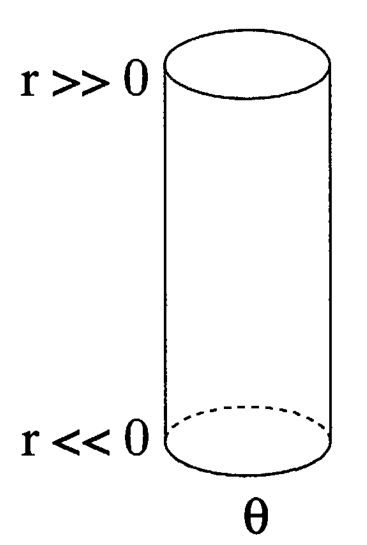
\includegraphics[width=0.28\textwidth]{figs/fig_p192_1.png}
  \caption{$t$ 柱面：顶部标 $r\gg0$（$\sigma$ 模型端），底部标 $r\ll0$（Landau--Ginzburg 端），绕柱圆周为 $\theta$ 角。（原文 Figure 8，p.192）}
  \label{fig:p192-1}
\end{figure}

现在详细考察这两种情形。
对 $k<n$，$\sigma$ 模型的目标空间是 Fano 簇，即 $\mathbf{CP}^{n-1}$ 中次数 $k<n$ 的超曲面。
这在紫外是一个好的描述，给出一个提法恰当的量子场论，其红外行为正是我们想确定的。
红外流把我们带到 $r\ll0$，在那里我们找到两类真空：(1) 中心荷为 $\widehat{c}=n(1-2/k)$ 的共形场论真空；(2) 大 $\sigma$ 处 $n-k$ 个新真空。
大 $\sigma$ 处相应的有效扭曲超势为
\[
\widetilde{\mathcal{W}}_{\rm eff}=t\Sigma+\frac{i}{2\pi}(n-k)(\Sigma-\Sigma\ln\Sigma).
\]
这两类真空的中心荷都小于紫外理论的值 $\widehat{c}=n-2$。
因此在这个例子中，单个紫外量子场论可以流向相当不同的红外可能性。
二维 $\mathcal{N}=2$ $\sigma$ 模型的重整化群流

% ===== 原文 p.193 =====

有许多不变量（例如 $\operatorname{Tr}(-1)^F$、椭圆亏格，以及它们的一些近亲）。
要重现 Fano 目标的紫外 $\sigma$ 模型的不变量，必须对 (1)、(2) 两类红外真空求和。

\subsubsection{$c_1<0$ 的情形}
% 原文 §13.6.5：The case $c_1<0$

现在考虑相反的情形 $k>n$。
$\mathbf{CP}^{n-1}$ 中次数 $k>n$ 的超曲面是一般型代数簇（algebraic variety of general type）。
此时 $\beta>0$，并且不存在一个定义良好的量子场论，其场是从时空到该超曲面的映射。
然而，以该超曲面为目标空间的 $\sigma$ 模型作为红外的有效理论是有意义的。
人们可以问：什么样的定义良好的紫外理论能在红外流到这个有效理论？

对这个问题，下面给出一个答案。
对 $k>n$，柱面的紫外稳定端是 Landau--Ginzburg 端。
Landau--Ginzburg 模型的中心荷为 $\widehat{c}=n(1-2/k)$，当 $k>n$ 时它大于 $\sigma$ 模型的值 $\widehat{c}=n-2$。
因此 Zamolodchikov 定理允许从 LG 模型到 $\sigma$ 模型的重整化群流。
这正是实际发生的，因为当 $n<k$ 时柱面上的重整化群流是「向上」的，即离开 LG 模型、趋向 $\sigma$ 模型。

% [Tutor Note: 这里的方向一致性可用 Zamolodchikov 定理直接自检：$k>n$ 时 $\widehat{c}_{\rm LG}=n(1-2/k)>n-2=\widehat{c}_\sigma$，故只允许 LG（紫外）$\to\sigma$（红外），反向流被禁止；而 $k<n$ 时不等式反转，只允许 $\sigma$（紫外，Fano）$\to$ LG（红外）。换句话说，「哪个端是紫外」完全由 $n-k$ 的符号决定，而不是由柱面上 $r$ 的符号决定——$r\gg0$ 永远对应 $\sigma$ 模型、$r\ll0$ 永远对应 LG，变的只是流的方向。]

若 $k>n$，在柱面的 LG 端没有大 $\sigma$ 真空。
取而代之，有 $k-n$ 个这样的真空伴随着 $\sigma$ 模型。
因此，由 Landau--Ginzburg 模型给出的一个定义良好的紫外不动点，可以在红外流向该超曲面的 $\sigma$ 模型，或流向大 $\sigma$ 处的非经典有质量真空。
正如 $k<n$ 的情形，要想在紫外与红外理论之间等同诸如 $\operatorname{Tr}(-1)^F$ 这样的重整化群不变量，必须对红外极限下的两类真空求和。

\begin{figure}[htbp]
  \centering
  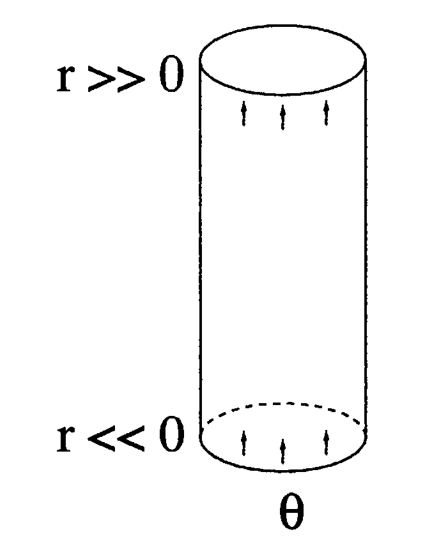
\includegraphics[width=0.28\textwidth]{figs/fig_p193_1.png}
  \caption{$t$ 柱面：与 Figure 8 相同的两个端（$r\gg0$ 在上、$r\ll0$ 在下），但柱面上的箭头改为向上，表示 $k>n$ 时重整化群流沿柱面「向上」，即从 LG 端流向 $\sigma$ 模型端。（原文 Figure 9，p.193）}
  \label{fig:p193-1}
\end{figure}

注意，无论 $n-k$ 的符号如何，非经典真空总是出现在红外而不是紫外。
这有一个很好的直观理由。
在紫外，也就是我们定义理论的地方，我们可以（在所有可能的紫外不动点中）挑选我们想研究的理论，所以紫外理论只有一类真空。
走向红外意味着解方程，而在这个阶段事情就不由我们作主了：一个确定的量子场论对其红外行为可以有不止一个解。
这正是我们今天所发现的。
事实上我们已经看到，一个确定的紫外场论（$k<n$ 时基于 Fano 簇，$k>n$ 时基于 Landau--Ginzburg 模型）可以流向相当不同的红外可能性。

% ===== 原文 p.194 =====

我们今天研究过的 $k\ne n$ 的两种情形都具有相当的方法论意义。
对 $k<n$，我们看到具有 Fano 目标的量子理论一般给出一种混合的答案：既有 Calabi--Yau 流形的行为，又有复射影空间的行为。
对 $k>n$，我们在一个具体情形中找到了一个定义良好的紫外不动点，它流向基于一般型代数簇的有效理论。

\subsection{参考文献与交叉引用}
% 原文 References and cross references

本材料的基本参考文献是
\begin{quote}
E. Witten, \emph{Phases of $\mathcal{N}=2$ SUSY theories in two dimensions}, Nucl. Phys. B \textbf{403} (1993), p.159--222.
\end{quote}

% [Tutor Note: 本页出现的几个交叉引用代号 $[I\text{-}\dots]$、$[II\text{-}\dots]$ 指本丛书第 I 卷（数学部分）与第 II 卷（物理部分）的对应章节，而非本文内部的编号，故原样保留。注意 [I-Renorm Groups] 即第 I 卷中关于重整化群的章节，其缩写为 ``Renorm Groups'' 而非 ``Renormalization Group''，检索时勿按全称拼写。]

CFT 的中心荷这一概念是在 [II-CFT, §2.4] 中引入的，在 [II-Strings] 的第 3 讲中也有讨论。
$\beta$ 函数与重整化群流在 [I-Renorm Groups] 的第 3 讲中有详细讨论。
关于我们可以加进超对称拉氏量的各种可能的项（包括 Fayet--Iliopoulos 项），在 [I-Supersolutions] 第 9 章中给出。

% [Tutor Note: 原文此句有两处排印讹误：一是 ``Fayet-Iliopulous''，正确拼法为 Fayet--Iliopoulos（P. Fayet 与 J. Iliopoulos, Phys. Lett. B 51 (1974) 461）；二是 ``are given is Chapter 9''，介词误作 ``is''，应为 ``in''。译文按正确拼法与语义处理；读者若按原文检索文献，应以 Fayet--Iliopoulos 为准。]

CFT 中极小模型的一个参考文献是
\begin{quote}
W. Boucher, D. Friedan, and A. Kent, \emph{Determinant formulae and unitarity for the $\mathcal{N}=2$ superconformal algebra in two dimensions, or exact results on string compactification}, Phys. Lett. B \textbf{172} (1986), p.~316.
\end{quote}

关于某些 Landau--Ginzburg 模型的红外极限与极小模型之间关系的讨论，见于
\begin{quote}
B. Greene, C. Vafa, and N. Warner, \emph{Calabi--Yau manifolds and renormalization group flows}, Nucl. Phys. B \textbf{324} (1989), p.~371--390.\\
E. Martinec, \emph{Criticality, catastrophes and compactifications}, in: L. Brink et al., eds., \emph{Physics and Mathematics of Strings}, World Scientific, 1990, p.~389--433.
\end{quote}

关于这一论断的更多证据见第 15 讲。

GIT（几何不变量理论，geometric invariant theory）的基本参考文献，以及关于 flop 在辛约化（symplectic reduction）背景下如何出现的文献，是
\begin{quote}
D. Mumford, J. Fogarty, and F. Kirwan, \emph{Geometric Invariant Theory}, Springer-Verlag, 1994.\\
V. Guillemin and S. Sternberg, \emph{Birational equivalence in the symplectic category}, Invent. Math \textbf{97} (1987), p.~485.\\
P. Aspinwall, B. Greene, and D. Morrison, \emph{Calabi--Yau moduli space, mirror manifolds and spacetime topology change in string theory}, Nucl. Phys. B \textbf{416} (1994), p.414--480.
\end{quote}

Zamolodchikov 定理的参考文献是
\begin{quote}
A. B. Zamolodchikov, \emph{`Irreversibility' of the flux of the renormalization group in a 2-D field theory}, JETP Lett. \textbf{43} (1986), pp.~730--732; Pisma Zh. Eksp. Teor. Fiz. \textbf{43} (1986), pp.~565--567. (Reprinted in Itzykson, C. (ed.) et al., \emph{Conformal invariance and applications to statistical mechanics}, pp.~702--704.)
\end{quote}
